\documentclass[12pt,fleqn]{article}\usepackage{../../common}
\begin{document}
Ders 17






























Ekler

Lorenz ODE Denklemlerinin Say�sal Olarak ��z�m�

\begin{minted}[fontsize=\footnotesize]{python}
import numpy as np
from scipy.integrate import odeint
def rhs(u,t,beta,rho,sigma):
    x,y,z = u
    return [sigma*(y-x), rho*x-y-x*z, x*y-beta*z]

sigma=10.0
beta=8.0/3.0
rho1=29.0
rho2=28.8

u01=[1.0,1.0,1.0]
u02=[1.0,1.0,1.0]

t=np.linspace(0.0,50.0,10001)
u1=odeint(rhs,u01,t,args=(beta,rho1,sigma))
u2=odeint(rhs,u02,t,args=(beta,rho2,sigma))

x1,y1,z1=u1[:, 0],u1[:, 1],u1[:, 2]
x2,y2,z2=u2[:, 0],u2[:, 1],u2[:, 2]

import matplotlib.pyplot as plt
from mpl_toolkits.mplot3d import Axes3D

fig=plt.figure()
ax=Axes3D(fig)
ax.plot(x1,y1,z1,'b-')
ax.plot(x2,y2,z2,'r:')
ax.set_xlabel('x')
ax.set_ylabel('y')
ax.set_zlabel('z')
ax.set_title('Lorenz denklemleri, rho = %g, %g' % (rho1,rho2))
plt.savefig('chaos_17_01.png')
\end{minted}

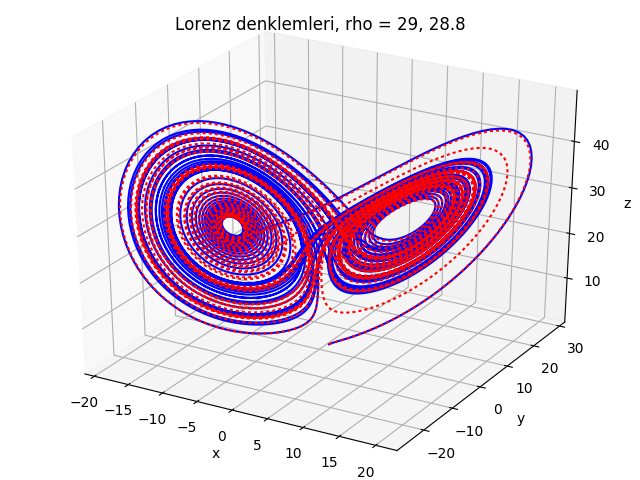
\includegraphics[height=6cm]{chaos_17_01.png}












Kaynaklar

[1] Saha, {\em 42 Problems in Scientific Computing}, \url{http://www.physik.uzh.ch/~psaha/teach/42probs.pdf}

\end{document}

